% Created 2017-09-19 Tue 17:09
% Intended LaTeX compiler: pdflatex
\documentclass[11pt]{article}
\usepackage[utf8]{inputenc}
\usepackage[T1]{fontenc}
\usepackage{graphicx}
\usepackage{grffile}
\usepackage{longtable}
\usepackage{wrapfig}
\usepackage{rotating}
\usepackage[normalem]{ulem}
\usepackage{amsmath}
\usepackage{textcomp}
\usepackage{amssymb}
\usepackage{capt-of}
\usepackage{hyperref}
\author{Francesco Ferraro, Diego Batista, Leonardo Martins}
\date{Setembro/2017}
\title{T1 Autômatos}
\hypersetup{
 pdfauthor={Francesco Ferraro, Diego Batista, Leonardo Martins},
 pdftitle={T1 Autômatos},
 pdfkeywords={},
 pdfsubject={},
 pdfcreator={Emacs 25.1.2 (Org mode 9.0.10)}, 
 pdflang={English}}
\begin{document}

\maketitle
\begin{abstract}
Entrega formal do primeiro trabalho da disciplina de automatos na PUCRS.
\end{abstract}

\section{Questão 1 - Cadeias}
\label{sec:orgc8980a8}
\subsection{Terminam por bcb}
\label{sec:org27c2dee}
\begin{figure}[htbp]
\centering
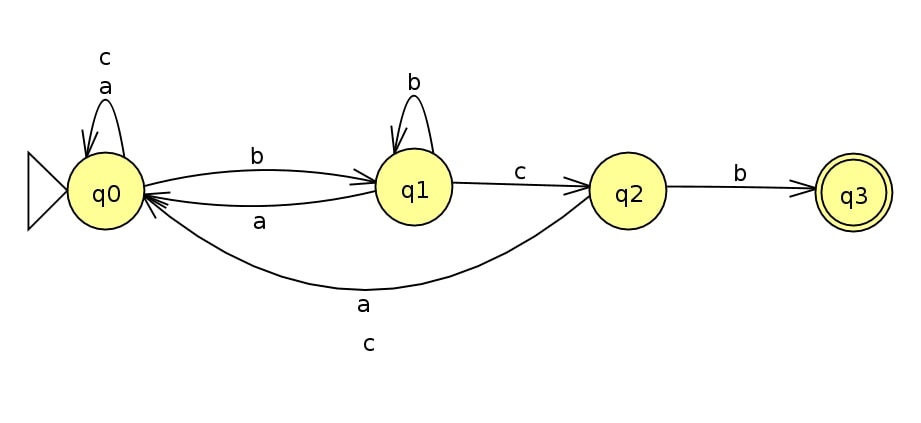
\includegraphics[width=.9\linewidth]{./q1/a/q1a.jpg}
\caption{\label{fig:org8710dfc}
Esse é um autômato determinístico}
\end{figure}

\begin{center}
\begin{tabular}{ll}
Input & Result\\
\hline
abcb & Accept\\
bcbb & Reject\\
cbcb & Accept\\
bcbaaa & Reject\\
aaaaa & Reject\\
\end{tabular}
\end{center}

\subsection{Terminam por no máximo dois b´s}
\label{sec:orgf04cae4}
\begin{figure}[htbp]
\centering
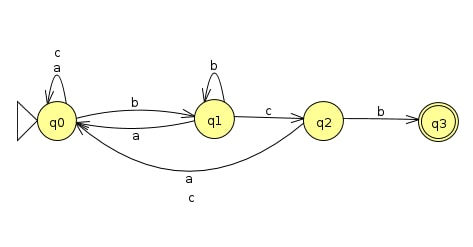
\includegraphics[width=.9\linewidth]{./q1/b/q1b.jpg}
\caption{\label{fig:org7b87976}
Esse é um autômato determinístico}
\end{figure}

\begin{center}
\begin{tabular}{ll}
Input & Result\\
\hline
b & Reject\\
a & Reject\\
c & Reject\\
bb & Reject\\
aba & Reject\\
ac & Reject\\
ab & Reject\\
bc & Reject\\
ba & Reject\\
\end{tabular}
\end{center}

\subsection{Não terminam por dois bs consecutivos}
\label{sec:orgbfe0133}
\begin{figure}[htbp]
\centering
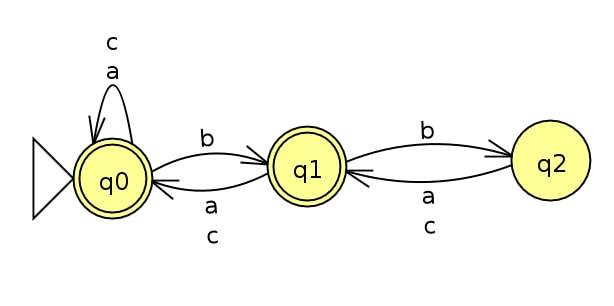
\includegraphics[width=.9\linewidth]{./q1/c/q1c.jpg}
\caption{\label{fig:orgb5ebb2f}
Esse é um autômato determinístico}
\end{figure}

\begin{center}
\begin{tabular}{ll}
Input & Result\\
\hline
aa & Accept\\
bb & Reject\\
cc & Accept\\
c & Accept\\
a & Accept\\
b & Accept\\
aacbac & Accept\\
abcabc & Reject\\
\end{tabular}
\end{center}
\subsection{Iniciam por a e terminam com c}
\label{sec:org0428ce1}
\begin{figure}[htbp]
\centering
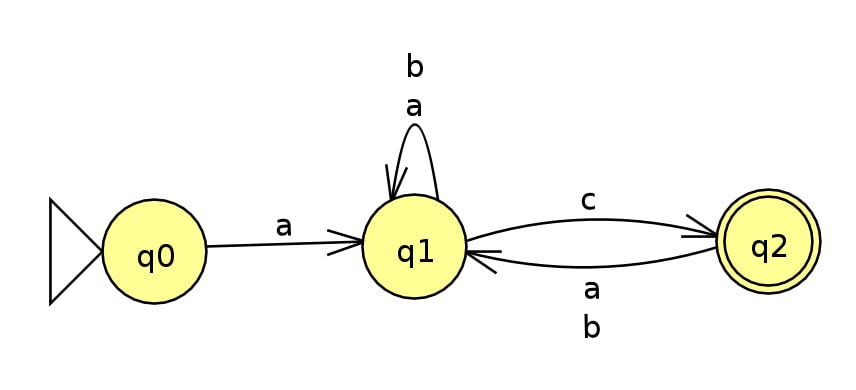
\includegraphics[width=.9\linewidth]{./q1/d/q1d.jpg}
\caption{\label{fig:orga308f42}
Esse é um autômato determinístico}
\end{figure}

\begin{center}
\begin{tabular}{ll}
Input & Result\\
\hline
a & Reject\\
b & Reject\\
c & Reject\\
ac & Accept\\
abcbc & Accept\\
acac & Accept\\
abcbb & Reject\\
\end{tabular}
\end{center}
\subsection{Iniciam e terminam pelo mesmo símbolo}
\label{sec:org9bc615b}
\begin{figure}[htbp]
\centering
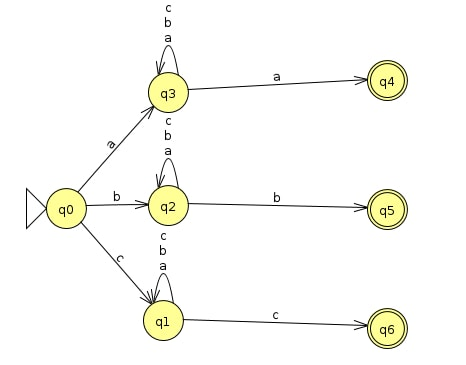
\includegraphics[width=.9\linewidth]{./q1/e/q1e.jpg}
\caption{\label{fig:org578475a}
Esse é um autômato determinístico}
\end{figure}

\begin{center}
\begin{tabular}{ll}
Input & Result\\
\hline
aa & Accept\\
bb & Accept\\
cc & Accept\\
ac & Reject\\
ab & Reject\\
bbaa & Reject\\
bba & Reject\\
\end{tabular}
\end{center}
\subsection{Iniciam e terminam por símbolos diferentes}
\label{sec:orgf7ca7c6}

\begin{figure}[htbp]
\centering
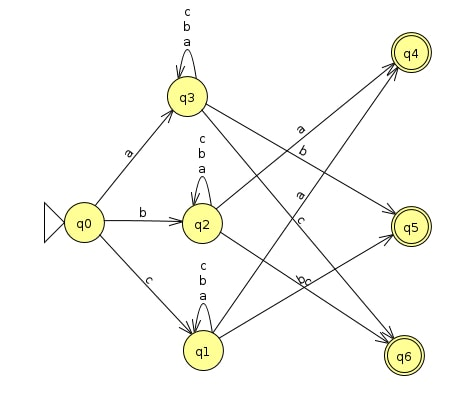
\includegraphics[width=.9\linewidth]{./q1/f/q1f.jpg}
\caption{\label{fig:orgd1779de}
Esse é um autômato determinístico}
\end{figure}

\begin{center}
\begin{tabular}{ll}
Input & Result\\
\hline
aa & Reject\\
bb & Reject\\
cc & Reject\\
ac & Accept\\
ab & Accept\\
bbaa & Accept\\
bba & Accept\\
abcbcba & Reject\\
\end{tabular}
\end{center}

\subsection{Número ímpar de b’s}
\label{sec:orgb0ff212}
\begin{figure}[htbp]
\centering
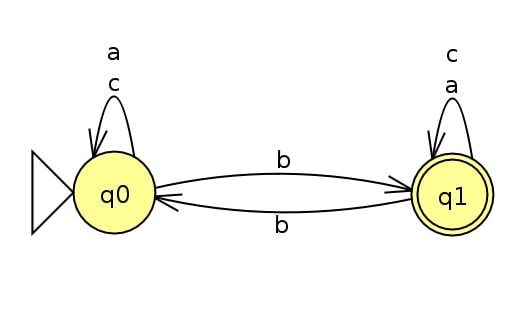
\includegraphics[width=.9\linewidth]{./q1/g/q1g.jpg}
\caption{\label{fig:orgb0686a9}
Esse é um autômato determinístico}
\end{figure}

\begin{center}
\begin{tabular}{ll}
Input & Result\\
\hline
aa & Reject\\
bb & Reject\\
cb & Accept\\
ac & Reject\\
ab & Accept\\
bbaa & Reject\\
bba & Reject\\
abcbcba & Accept\\
b & Accept\\
\end{tabular}
\end{center}
\section{Questão 2 - Expressões Regulares}
\label{sec:org188f41d}
\subsection{Terminam por 101}
\label{sec:orgf9b054f}

\begin{quote}
(0+1)*(101)
\end{quote}

\subsection{Iniciam por 1 e terminam com 0}
\label{sec:org1515c3d}

\begin{quote}
1(1+0)*0 
\end{quote}

\subsection{Iniciam e terminam pelo mesmo símbolo}
\label{sec:org142ed9a}

\begin{quote}
1(1+0)*1 + 0(1+0)*0 
\end{quote}

\subsection{Iniciam e terminam por símbolos diferentes}
\label{sec:org1c1ce7c}

\begin{quote}
1(1+0)*0 + 0(1+0)*1 
\end{quote}

\subsection{{\bfseries\sffamily TODO} Falta Uma}
\label{sec:orga70b434}

ER 

\section{Questão 3 - 10n1}
\label{sec:org8c8d310}
\subsection{Automato}
\label{sec:org3a87f93}
A figura \ref{fig:org86f7852} reponde essa questão. 

\begin{figure}[htbp]
\centering
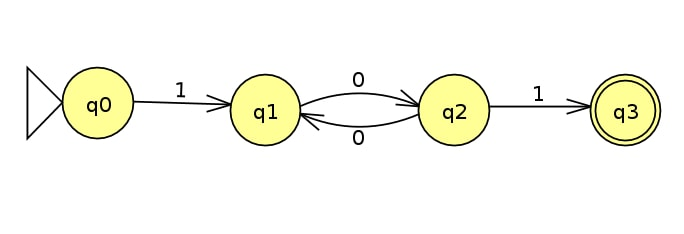
\includegraphics[width=.9\linewidth]{./q3/q3.jpg}
\caption{\label{fig:org86f7852}
Esse é um autômato determinístico}
\end{figure}

\begin{center}
\begin{tabular}{rl}
Input & Result\\
\hline
0 & Reject\\
01 & Reject\\
1 & Reject\\
101 & Accept\\
1001 & Reject\\
10001 & Accept\\
100001 & Reject\\
1000001 & Accept\\
10000001 & Reject\\
\end{tabular}
\end{center}
\subsection{Expressão regular}
\label{sec:orgdf778ce}

\textbf{10+(00)*+1} 
\section{{\bfseries\sffamily TODO} Questão 4 - AFND -> AFD}
\label{sec:org7cc3d5a}
Aqui vai uma super resolução.
\begin{figure}[htbp]
\centering
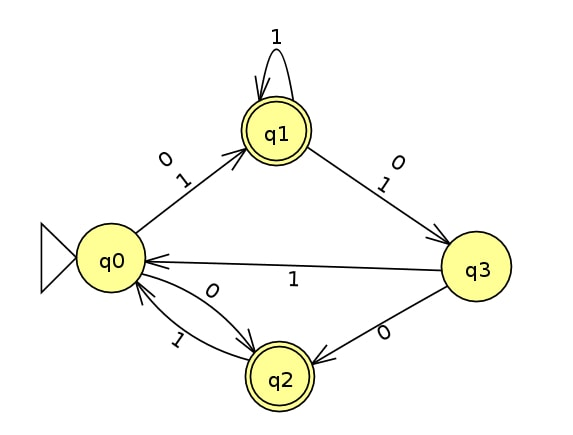
\includegraphics[width=.9\linewidth]{./q4/q4.jpg}
\caption{\label{fig:orgc5d32f2}
Esse é um autômato determinístico}
\end{figure}
\section{Questão 5  - V ou F}
\label{sec:org6b33128}
\subsection{Falso}
\label{sec:org7d1f713}
Uma vez que consumidas todas as entradas o AFND acaba com a execução ainda que a transição do vazia para o mesmo estado ocorra.  O fato de que o estado anterior a ela ser o mesmo que o posterior não faz o autômato entrar em loop.
\subsection{Verdadeira}
\label{sec:org71724cc}
\subsection{Falso}
\label{sec:org060fea4}
Um ADF sem ao menos 1 estado final reconhece só a linguagem vazia.
\subsection{Falsa}
\label{sec:orgb332003}
Por definição um AFD e AFND tem igual poder de reconhecimento

\pagebreak
\section{Questão 6 - Estacionamento}
\label{sec:orgf1860ee}
Resposta é a figura \ref{fig:org8afd675}.
\begin{figure}[htbp]
\centering
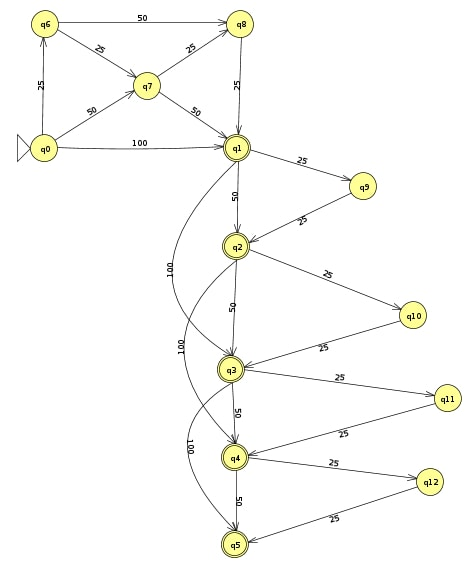
\includegraphics[width=.9\linewidth]{./q6/estacionamento.jpg}
\caption{\label{fig:org8afd675}
Autômato de uma parquímetro}
\end{figure}
\pagebreak
\section{{\bfseries\sffamily TODO} Questão 7 - Sinaleira}
\label{sec:org0432f5f}
\subsection{Analisando os semáforos paralelamente.}
\label{sec:org0d34b3e}

Resposta é a figura \ref{fig:orgb5ffb73}.
\begin{figure}[htbp]
\centering
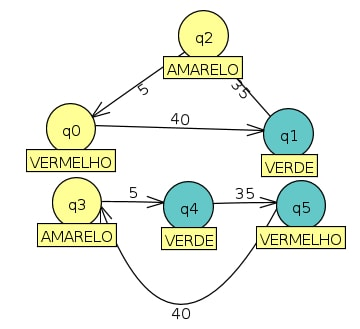
\includegraphics[width=.9\linewidth]{./q7/paralelo.jpg}
\caption{\label{fig:orgb5ffb73}
Autômato em paralelo}
\end{figure}

\subsection{Analisando os semáforos simultaneamente.}
\label{sec:org27e96fb}

Resposta é a figura \ref{fig:org3a54f2f}.
\begin{figure}[htbp]
\centering
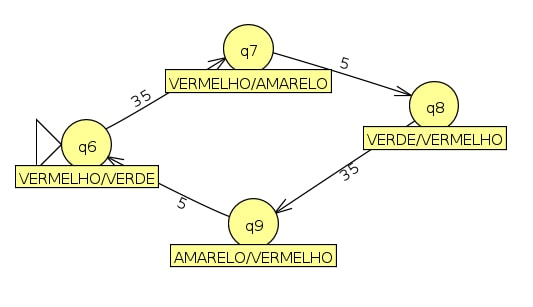
\includegraphics[width=.9\linewidth]{./q7/simultaneo.jpg}
\caption{\label{fig:org3a54f2f}
Autômato simultâneo}
\end{figure}
\end{document}
